\documentclass[12pt]{article}
\usepackage{amsmath}
\usepackage{amssymb}
\usepackage[letterpaper,margin=0.85in,centering]{geometry}
\usepackage{fancyhdr}
\usepackage{enumerate}
\usepackage{lastpage}
\usepackage{multicol}
\usepackage{graphicx}

\reversemarginpar

\pagestyle{fancy}
\cfoot{Page \thepage \ of \pageref{LastPage}}\rfoot{{\bf Total Points: 40}}
\chead{MATH 1010A}\lhead{Test \# 1}\rhead{Monday, 19\textsuperscript{th} October, 2015}

\newcommand{\points}[1]{\marginpar{\hspace{24pt}[#1]}}
\newcommand{\skipline}{\vspace{12pt}}
%\renewcommand{\headrulewidth}{0in}
\headheight 30pt

\newcommand{\di}{\displaystyle}
\newcommand{\R}{\mathbb{R}}
\newcommand{\aaa}{\mathbf{a}}
\newcommand{\bbb}{\mathbf{b}}
\newcommand{\ccc}{\mathbf{c}}
\newcommand{\dotp}{\boldsymbol{\cdot}}
\newcommand{\abs}[1]{\lvert #1\rvert}
\newcommand{\len}[1]{\lVert #1\rVert}
\newcommand{\ivec}{\,\boldsymbol{\hat{\imath}}}
\newcommand{\jvec}{\,\boldsymbol{\hat{\jmath}}}
\newcommand{\kvec}{\,\boldsymbol{\hat{k}}}
\DeclareMathOperator{\comp}{comp}

\begin{document}

\author{Instructor: Sean Fitzpatrick}
\thispagestyle{plain}
\begin{center}
\emph{University of Lethbridge}\\
Department of Mathematics and Computer Science\\
19\textsuperscript{th} October, 2015, 4:00 - 4:50 pm\\
{\bf MATH 1010A - Test \#1}\\
\end{center}
\skipline \skipline \skipline \noindent \skipline
Last Name:\underline{\hspace{50pt}{\bf Solutions}\hspace{248pt}}\\
\skipline
First Name:\underline{\hspace{50pt}{\bf The}\hspace{275pt}}\\
\skipline
Student Number:\underline{\hspace{323pt}}\\
\skipline
Tutorial Section: \underline{\hspace{320pt}}\\


\vspace{0.5in}


\begin{quote}
 {\bf Record your answers below each question in the space provided.    Left-hand pages may be used as scrap paper for rough work.  If you want any work on the left-hand pages to be graded, please indicate so on the right-hand page.
 
 \bigskip
 
Partial credit will be awarded for partially correct work, so be sure to show your work, and include all necessary justifications needed to support your arguments.

\bigskip

No external aids are allowed, with the exception of a 5-function calculator.}
\end{quote}


\vspace{0.5in}

For grader's use only:

\begin{table}[hbt]
\begin{center}
\begin{tabular}{|l|r|} \hline
Page&Grade\\
\hline \hline
\cline{1-2} 2 & \enspace\enspace\enspace\enspace\enspace\enspace/10\\
\cline{1-2} 3 & \enspace\enspace\enspace\enspace\enspace\enspace/10\\
\cline{1-2} 4 & \enspace\enspace\enspace\enspace\enspace\enspace/10\\
\cline{1-2} 5 & \enspace\enspace\enspace\enspace\enspace\enspace/10\\
\cline{1-2} Total & \enspace\enspace\enspace\enspace\enspace\enspace/40\\
\hline
\end{tabular}

\skipline

\skipline

\skipline

B
\end{center}
\end{table}
\newpage


\begin{enumerate}
\item Simplify the following expressions. Your final answer should be in the form $\dfrac{A}{B}$, where $A$ and $B$ are integers.
\begin{enumerate}
 \item $\dfrac{1-\left(\frac{3}{5}\right)\left(\frac{5}{9}\right)}{1+\left(\frac{3}{5}\right)\left(\frac{5}{9}\right)}$. \points{3}

\bigskip

\[
 \frac{1-\left(\dfrac{3}{\not 5}\right)\left(\dfrac{\not 5}{9}\right)}{1+\left(\dfrac{3}{\not 5}\right)\left(\dfrac{\not 5}{9}\right)} = \frac{1-\dfrac{3}{9}}{1+\dfrac{3}{9}} = \frac{1-\dfrac{1}{3}}{1+\dfrac{1}{3}} = \frac{\dfrac{2}{3}}{\dfrac{4}{3}}=\left(\frac{2}{\not 3}\right)\left(\frac{\not 3}{4}\right) = \frac{2}{4} = \frac{1}{2}.
\]

\bigskip

 \item $\left(\dfrac{64}{125}\right)^{-2/3}$. \points{3}

\bigskip

\[
 \left(\frac{64}{125}\right)^{-2/3} = \left(\frac{125}{64}\right)^{2/3} = \frac{(5^3)^{2/3}}{(4^3)^{2/3}} = \frac{5^2}{4^2} = \frac{25}{16}.
\]

\bigskip

\end{enumerate}
\item Simplify the following expression. Your final answer should be in the form $\dfrac{A}{B}$, where $A$ and $B$ are polynomials.\points{4} 

\[
\di \frac{x+1}{2+x}+\frac{2x}{2-x}-\frac{5x+6}{4-x^2} 
\]

\bigskip

\begin{align*}
 \frac{x+1}{2+x}+\frac{2x}{2-x}-\frac{5x+6}{4-x^2}&= \frac{(x+1)(2-x)}{(2+x)(2-x)}+\frac{2x(2+x)}{(2+x)(2-x)}-\frac{5x+6}{4-x^2}\\
& = \frac{(x+1)(2-x)+2x(2+x)-(5x+6)}{4-x^2}\\
& = \frac{-x^2+x+2+4x+2x^2-5x-6}{4-x^2}\\
& = \frac{x^2-4}{4-x^2} = -1.
\end{align*}

\newpage

\item Solve the following inequalities:
\begin{enumerate}
 \item $\dfrac{3}{4}-x \leq \dfrac{6x-2}{3}$. \points{3}

\bigskip

Dividing by 3 on the right-hand side, we have $\dfrac{3}{4}-x \leq 2x-\dfrac{2}{3}$. Adding $x$ to both sides to bring all the terms involving $x$ to the right, and adding $\dfrac{2}{3}$ to both sides to bring all constant terms to the left, we obtain
\[
 \dfrac{3}{4}+\dfrac{2}{3}\leq 3x.
\]
Since $\dfrac{3}{4}+\dfrac{2}{3} = \dfrac{9}{12}+\dfrac{8}{12} = \dfrac{17}{12}$, we have $\dfrac{17}{12}\leq 3x$, and dividing both sides by $3$ (noting that $3>0$), we have
\[
 \frac{17}{36}\leq x \quad \text{ or } \quad x\geq \frac{17}{36}. \quad \text{ In interval notation, } \quad x\in \left[\frac{17}{36},\infty\right).
\]

\bigskip

 \item $5x\geq 2-x\geq 0$ \points{4}

\bigskip

We are given a pair of inequalities. The first one is $5x\geq 2-x$; adding $x$ to both sides gives us $6x\geq 2$, and dividing by 6, we find that $x\geq \dfrac{1}{3}$.

The second inequality is $2-x\geq 0$, which simplifies to $2\geq x$, or $x\leq 2$. Since we must satisfy {\bf both} inequalities, we must have $\dfrac{1}{3}\leq x$ {\bf and} $x\leq 2$, so $\dfrac{1}{3}\leq x\leq 2$. In interval notation, our solution is $x\in [\frac{1}{3},2]$.

\bigskip

 \item $\lvert 2x+1\rvert <5$ \points{3}

\bigskip

We recall that the statement $\lvert a\rvert \leq b$ is equivalent to $-b\leq a\leq b$ for any $a\in \mathbb{R}$ and any $b>0$. For the given inequality this gives us
\[
 -5\leq 2x+1\leq 5.
\]
Subtracting 1 from all three parts of this compound inequality yields $-6\leq 2x\leq 4$, and if we divide throughout by $2>0$, we obtain $-3< x\leq 2$. Thus we must have
$x\in (-3,2).$
\end{enumerate}
\newpage

\item Consider the function $f(x) = -x\lvert x\rvert$.
\begin{enumerate}
 \item Evaluate the following: $f(2), f(2) + f(-1), f(-2)\cdot f(3)$. \points{3}

\bigskip

We recall that $\lvert x\rvert = \begin{cases} x, & \text{ if } x\geq 0\\ -x, & \text{ if } x<0\end{cases}$, so that, for example, $\lvert 2\rvert = 2$, since $2>0$, while $\lvert -2\rvert = -(-2) = 2$, since $2<0$. (Note that $\lvert x\rvert \geq 0$ for all $x\in\mathbb{R}$.) Thus, we can compute as follows:
\[
 f(2) = -2\abs{2} = -2(2)=-4. \quad f(2)+f(-1) = -2\abs{2}+(-(-1))\abs{-1} = -2(2)+1(1) = -4+1=-3. 
\]
\[
 f(-2)\cdot f(3) = (-(-2)\abs{-2})((-3)\abs{-3}) = 2(2)(-3)(3) = -36.
\]

 \item Sketch the graph of $f$. (Hint: consider the cases $x\geq 0$ and $x<0$.) \points{3}

\begin{multicols}{2}
 For $x\geq 0$, we have $\abs{x}=x$, so $f(x)=-x\abs{x} = -x(x)=-x^2$. For $x<0$, $\abs{x}=-x$, so $f(x) = -x(-x)=x^2$. Thus our graph should consists of the part of the parabola $y=-x^2$ for $x\geq 0$, and the parabola $y=x^2$, for $x<0$, giving us the graph on the right:
\columnbreak
\begin{center}
 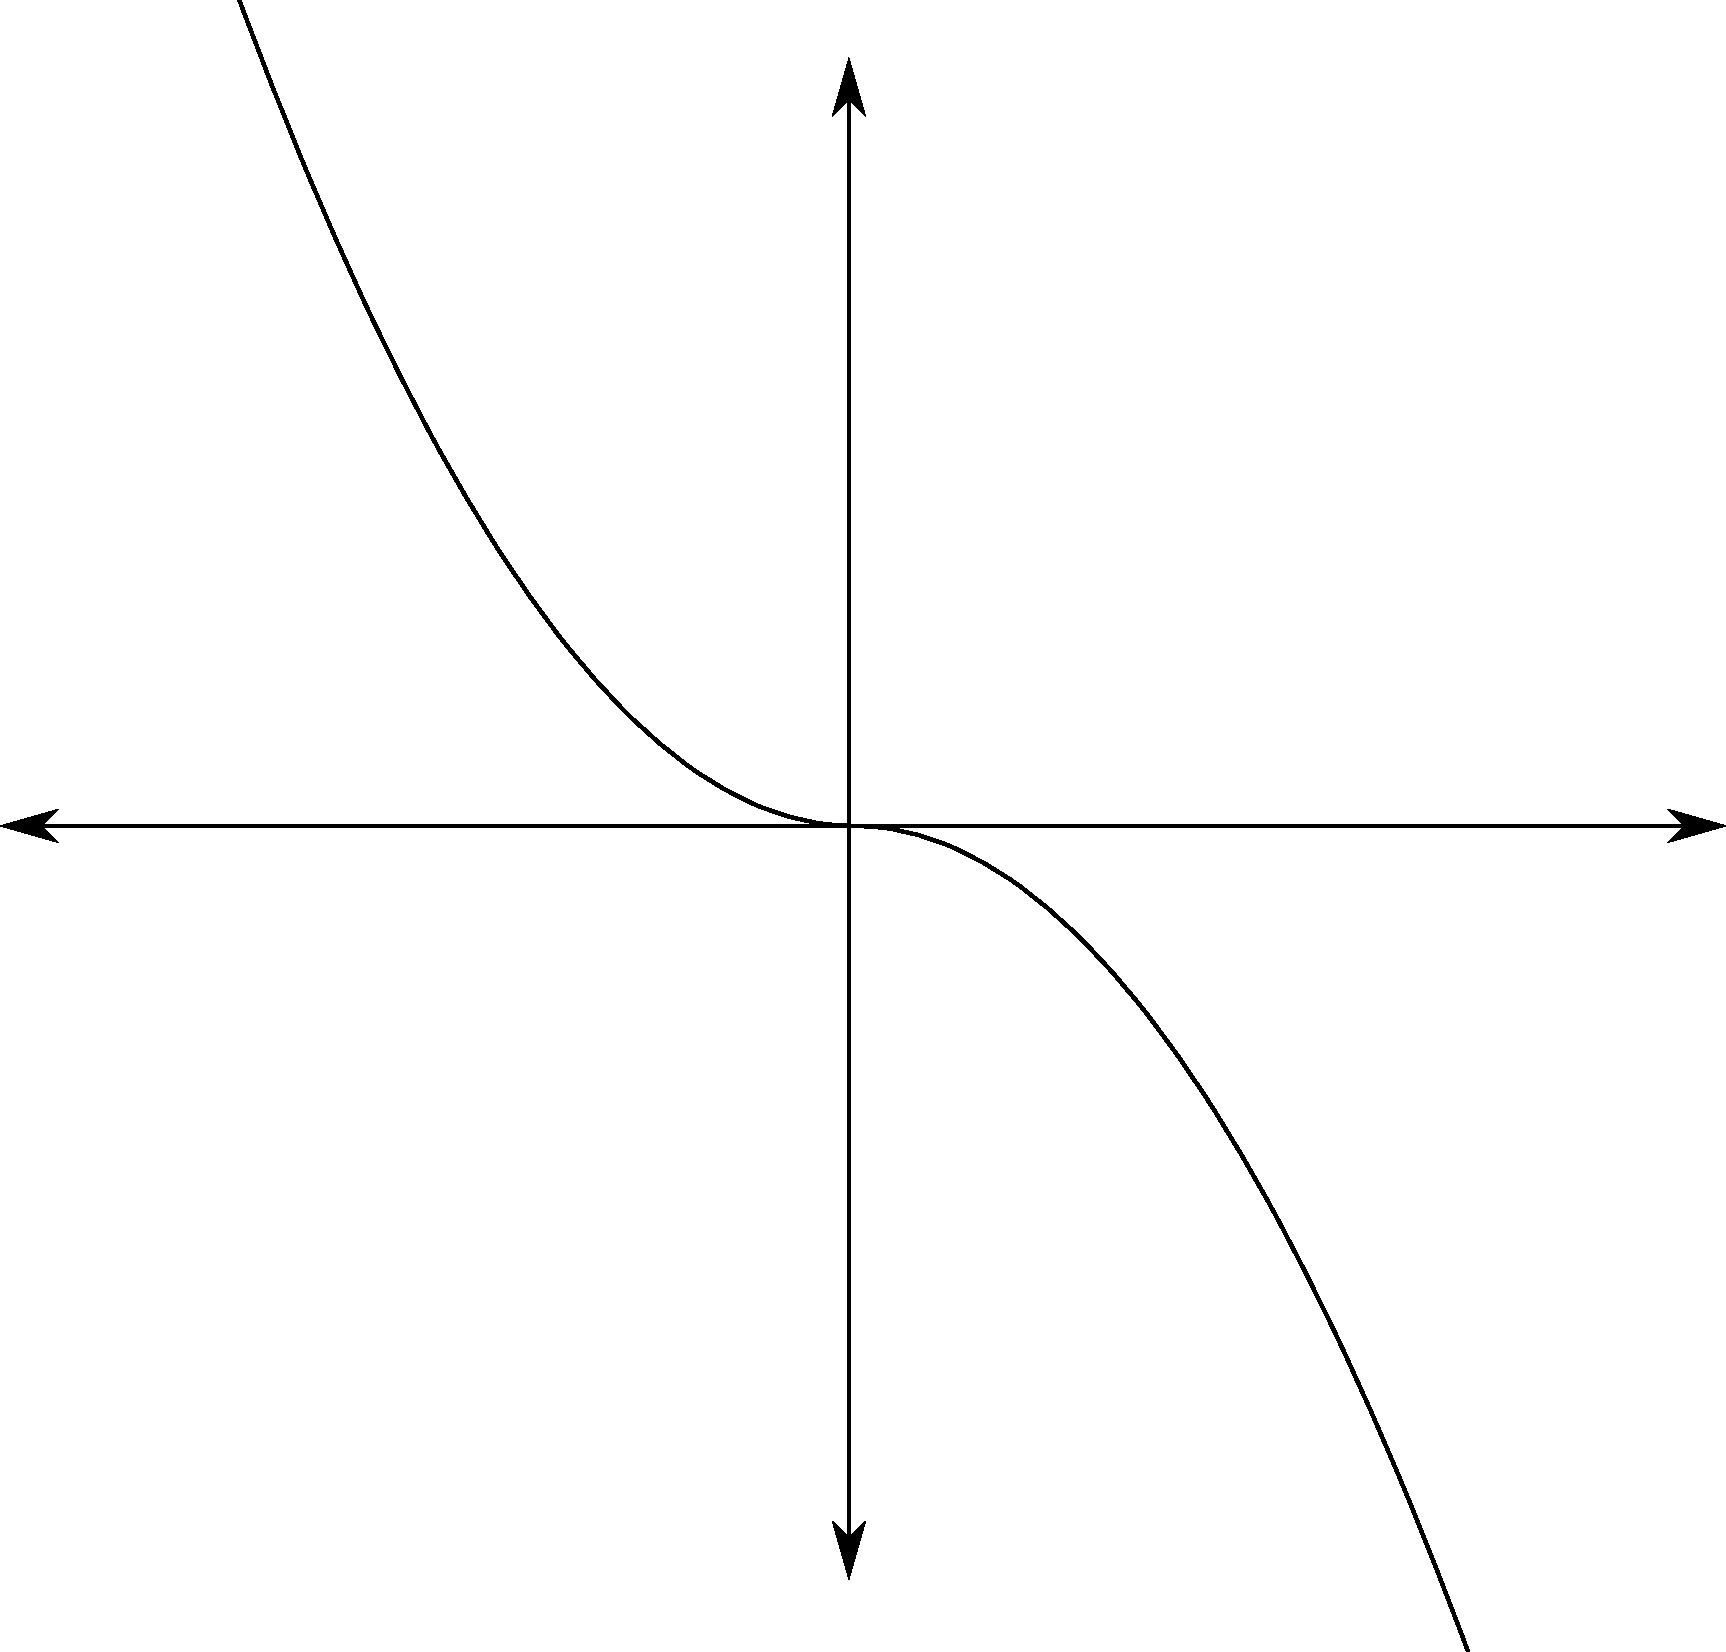
\includegraphics[height=2.3in]{Plot4(b)B.pdf}
\end{center}

\end{multicols}


 \item Sketch the graphs $y=f(x-3)$ and $y=-\frac{1}{3}f(x)+1$. \points{4}

{\bf Note:} if your graph in part (b) is incorrect, credit will be awarded for correct transformations of an incorrect graph.

\begin{multicols}{2}
 \begin{center}
 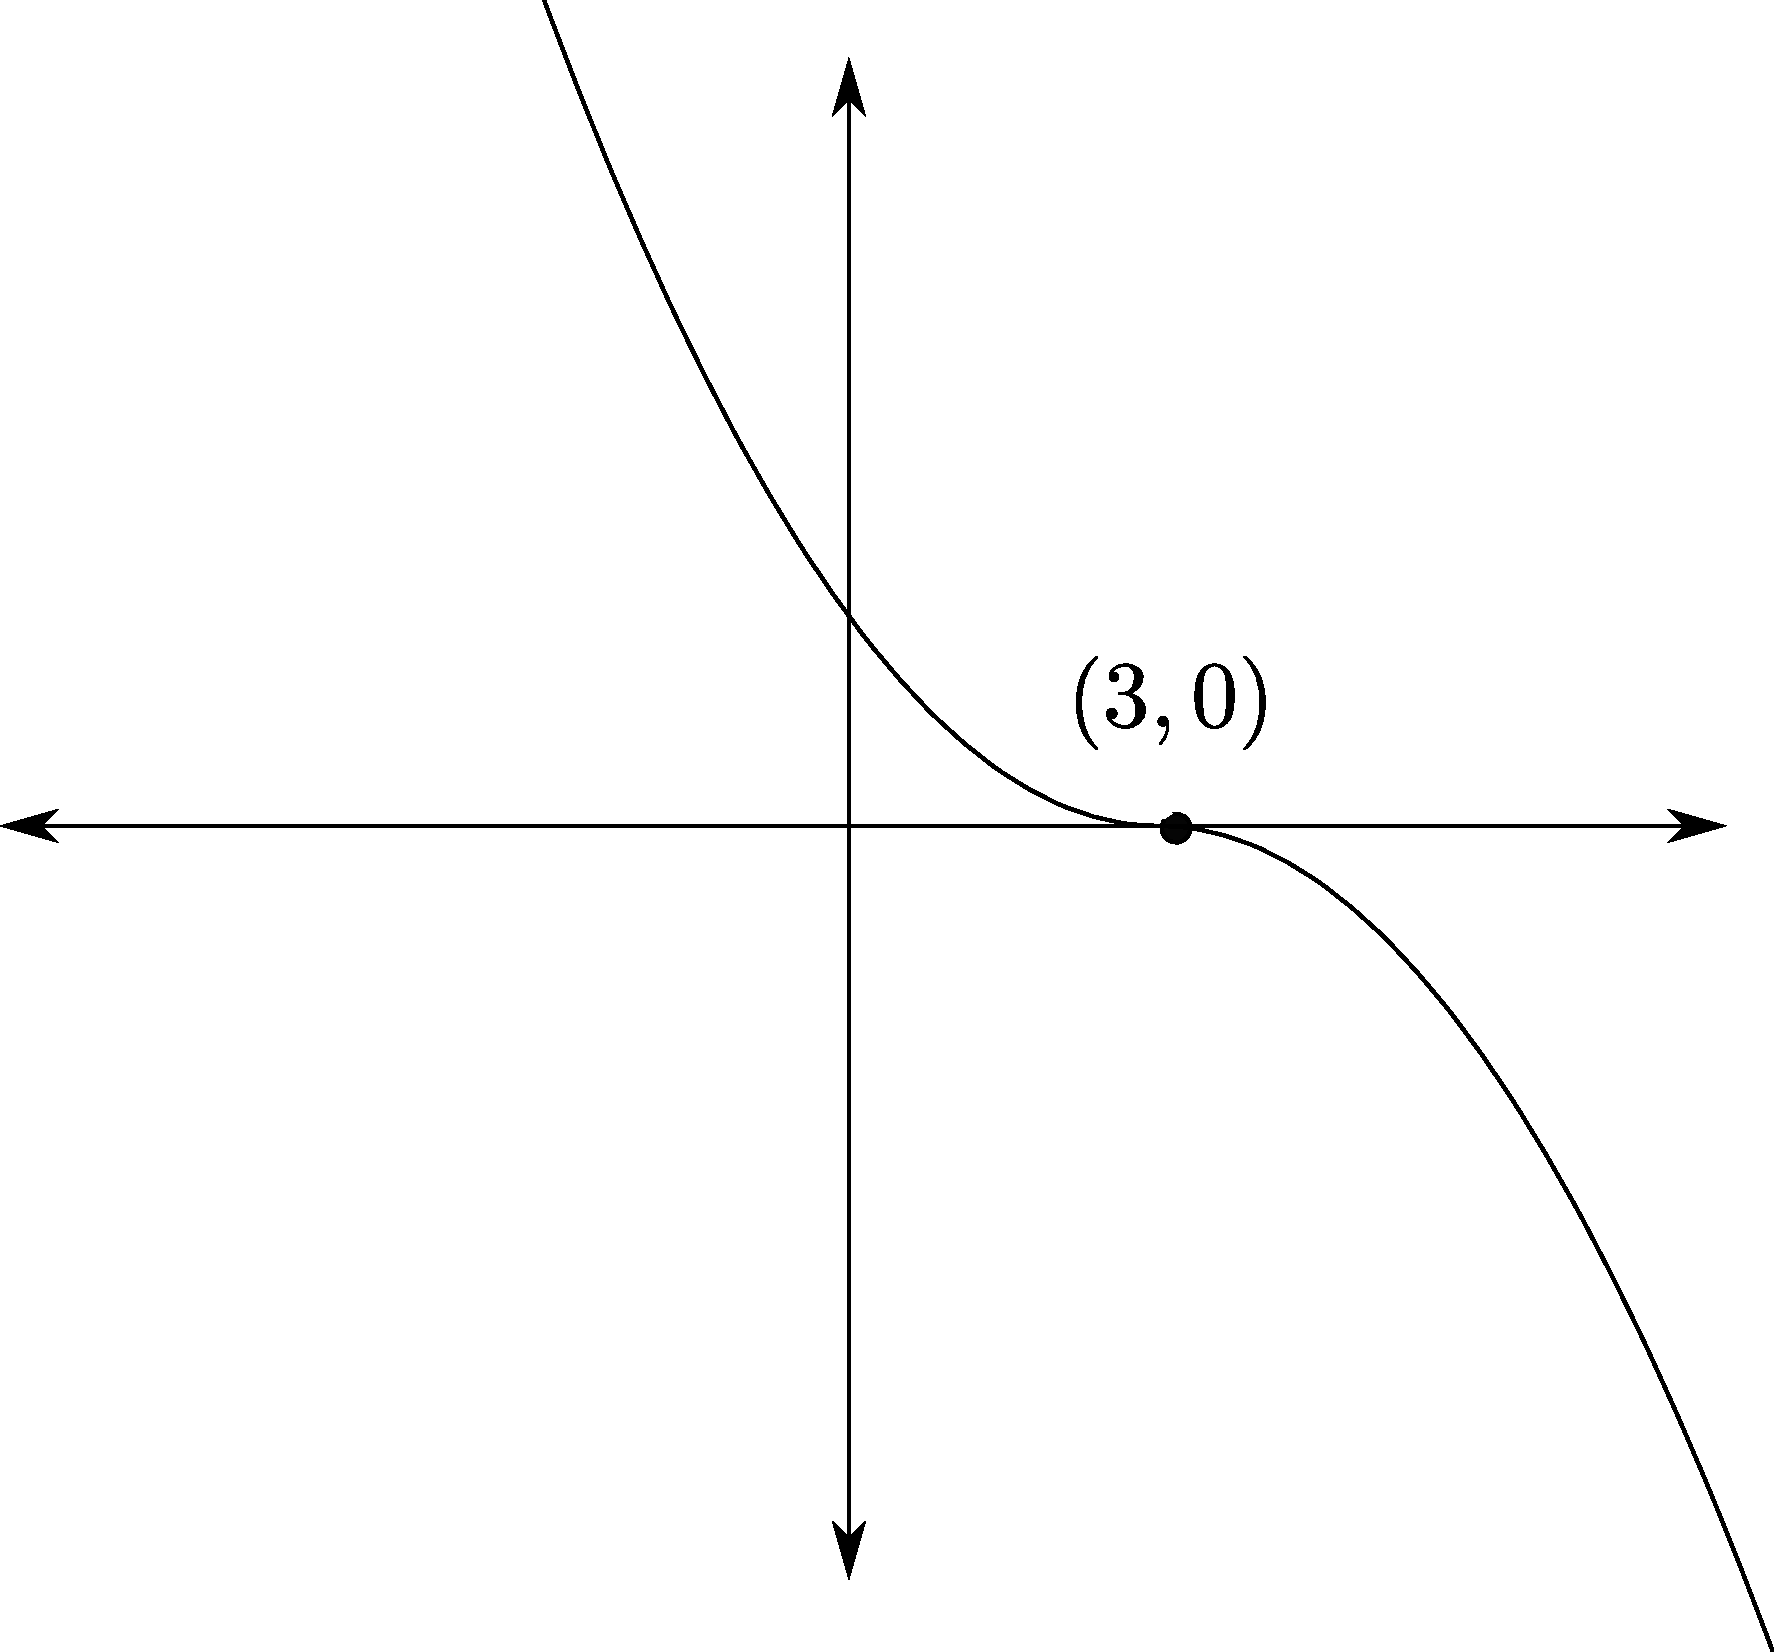
\includegraphics[height=2.5in]{Plot4(c)1B.pdf}

$y=f(x-3)$\\
This is a shift three units to the right.
\end{center}
\begin{center}
 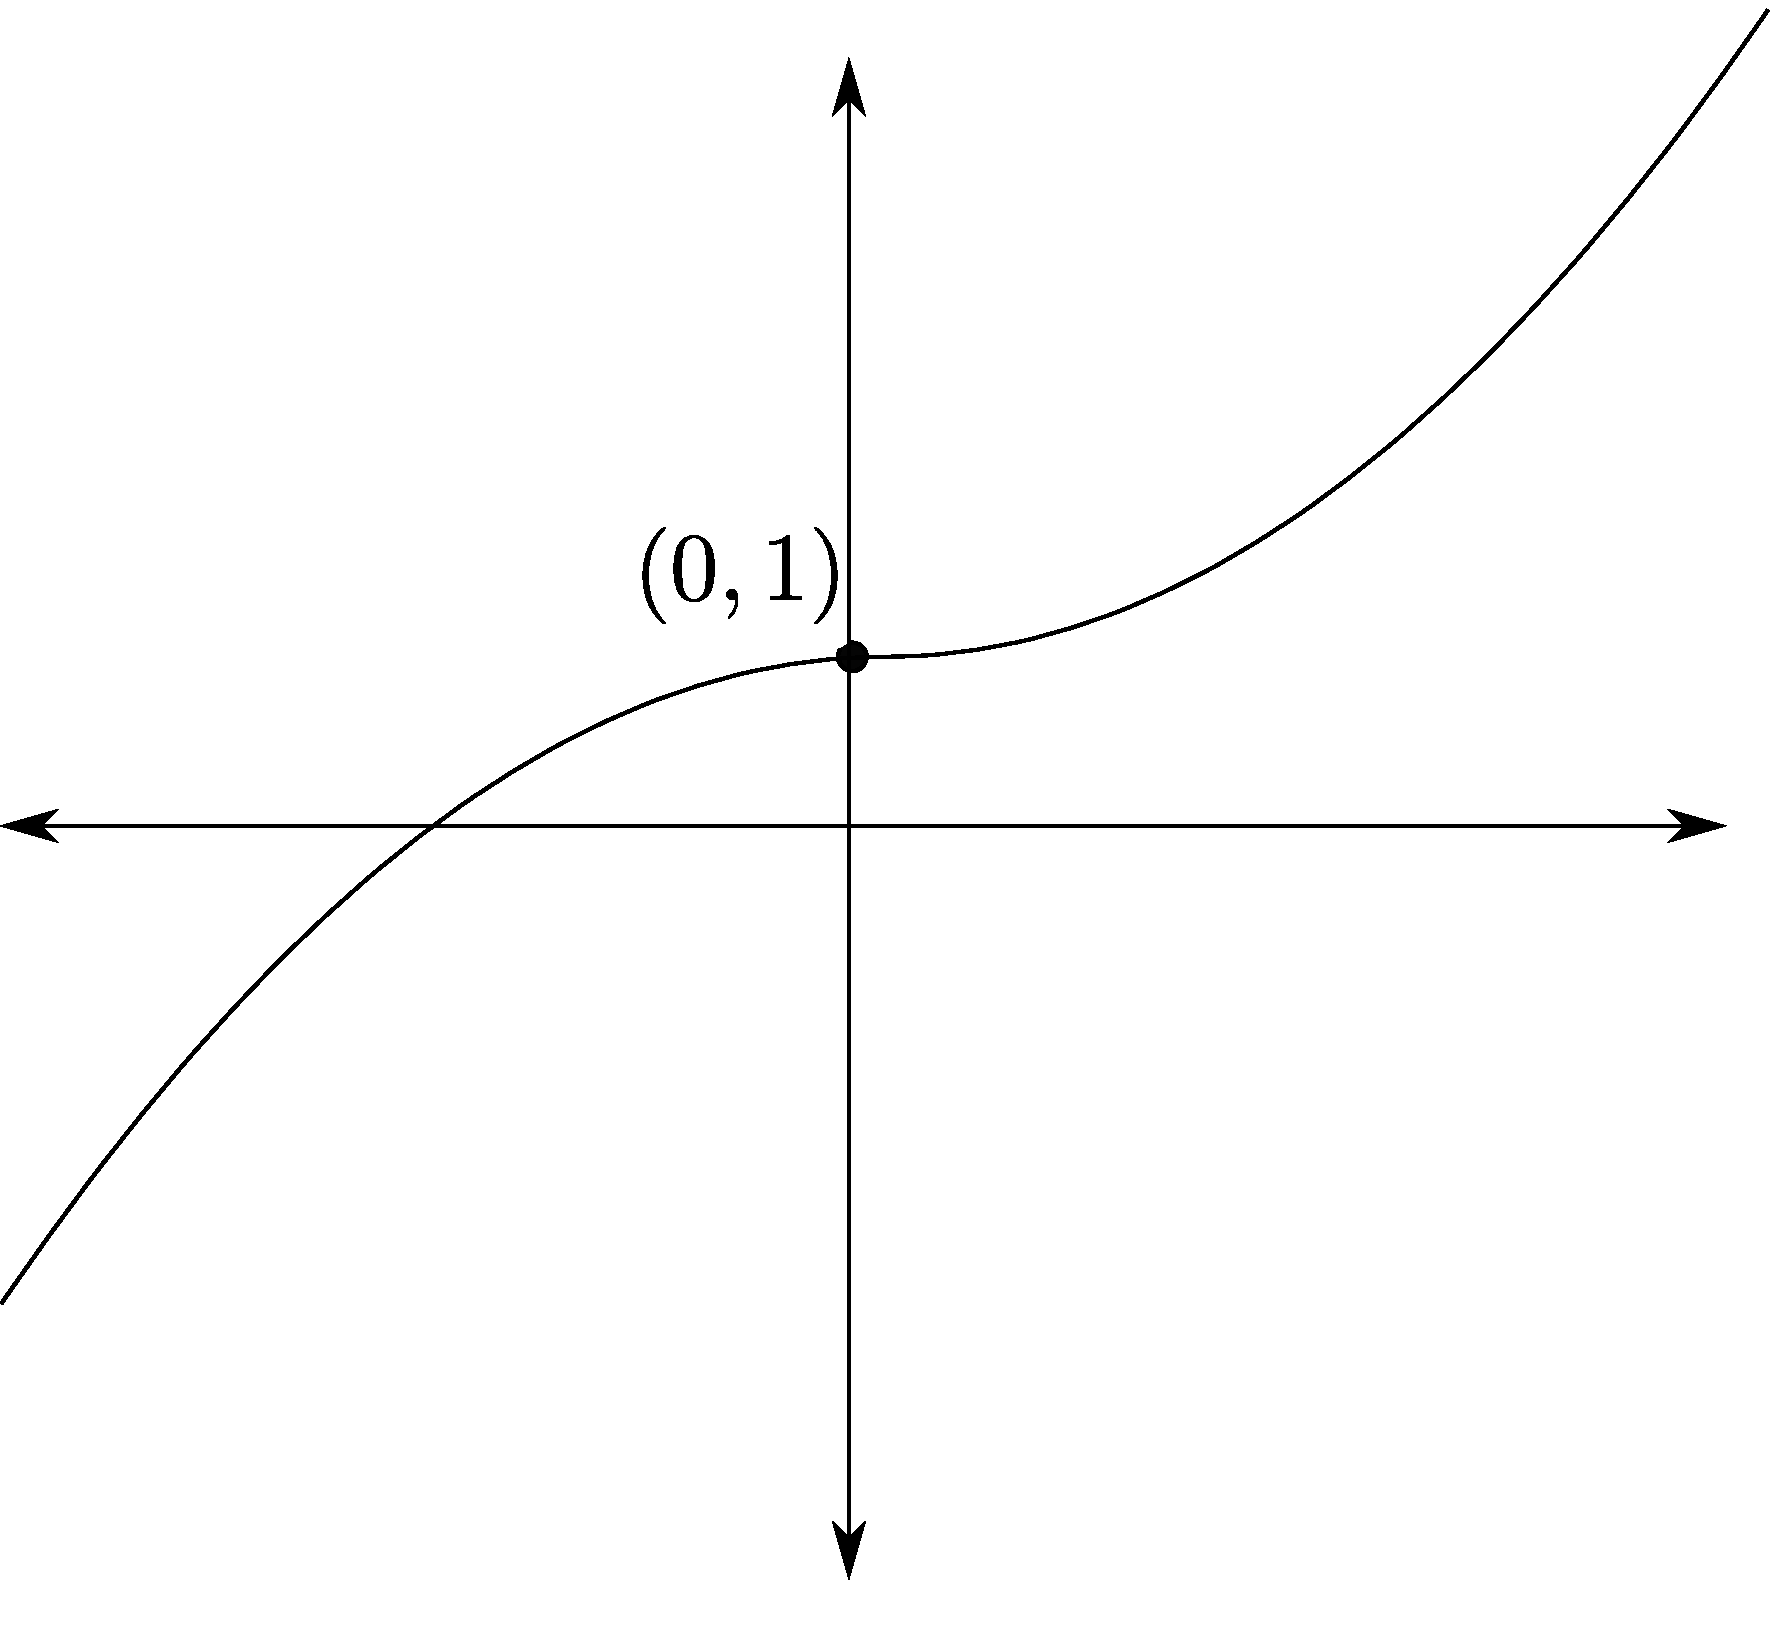
\includegraphics[height=2.5in]{Plot4(c)2B.pdf}

$y=-\frac{1}{3}f(x)+1$\\
This is a reflecion across the $x$-axis, followed by a vertical scaling by $1/3$, and a shift one unit up.
\end{center}
\end{multicols}

\end{enumerate}
\newpage

\item Consider the function $f(x) = x^2+4x-12$.
\begin{enumerate}
 \item Determine the sign diagram for $f$. \points{4}

\bigskip

We have $f(x) = x^2+4x-12 = (x+6)(x-2)$, so $f$ has zeros at $x=-6$ and $x=2$. We check that for $x>2$, $x+6>0$ and $x-2>0$, so $f(x)>0$. For $-6<x<2$, $x+6>0$ but $x-2<0$, so $f(x)<0$. For $x<-6$, $x+6<0$ and $x-2<0$, so $f(x)>0$. This gives us the sign diagram as follows:

\begin{center}
 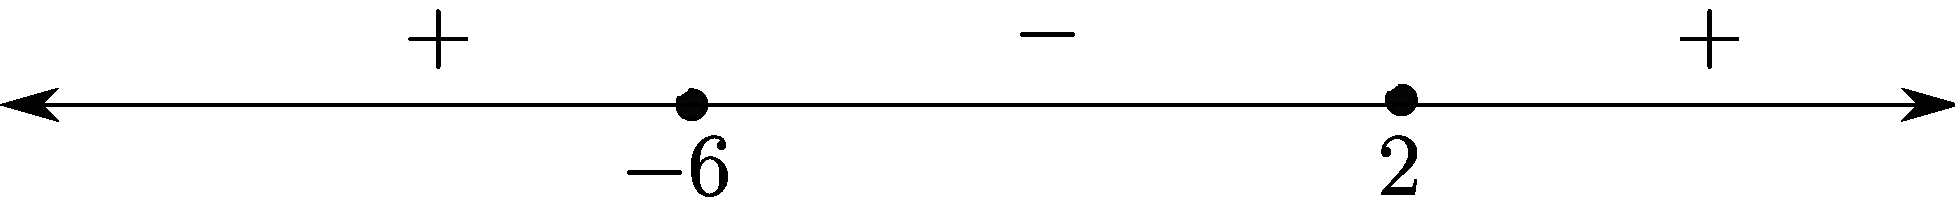
\includegraphics[width=4in]{SD5(a)B.pdf}
\end{center}

 \item Using your answer from part (a), solve the following:
\begin{enumerate}
 \item $f(x)=0$. \points{1}

\bigskip

From the sign diagram, we immediately see that $x^2+4x-12=0$ when\\ $x=-6$ or $x=2$.


\bigskip

 \item $f(x)\geq 0$. \points{1}
\end{enumerate}


\bigskip

Since the regions where $f(x)\geq 0$ correspond to the zeros and the intervals on the sign diagram with + signs, we immediately see that $f(x)\geq 0$ for\\ $x\in (-\infty, -6]\cup [2,\infty)$.

\bigskip


\item Since $f$ is a quadratic function, its graph is a parabola. Determine the location of the vertex of the parabola, as well as any $x$ or $y$-intercepts. (You do not have to sketch the graph.) \points{3}
\bigskip

We already have from part (b) that the $x$-intercepts are at $(-6,0)$ and $(2,0)$. Setting $x=0$ gives us $f(0)=-12$, so the $y$-intercept is at $(0,-12)$. To find the vertex, we complete the square to put $f$ in the ``vertex form'' as follows:
\[
 f(x) = x^2+4x-12 = (x^2+4x+4)-4-12 = (x+2)^2-16.
\]
From this, we can immediately conclude that the location of the vertex is the point $(-2,-16)$.

\bigskip


\item What is the domain of the function $g(x) = \dfrac{1}{\sqrt{12-4x-x^2}}$? \points{1}


\bigskip

In order for $g(x)$ to be defined, the denominator must be nonzero, and the polynomial under the square root cannot be negative. This leads to the condition $12-4x-x^2>0$, which is equivalent to $x^2+4x-12<0$, or $f(x)<0$, where $f$ is our function from part (a). From the sign diagram, we can immediately conclude that $f(x)<0$ for $x\in (-6,2)$, so the domain of $g$ is the open interval $(-6,2)$.


\end{enumerate}


\end{enumerate}
\end{document}